\documentclass[a4paper,11pt]{article}

\usepackage[utf8]{inputenc}
\usepackage[T1]{fontenc}
\usepackage[brazil]{babel}
\usepackage{amsmath,amssymb}
\usepackage{graphicx}
\usepackage{geometry}
\usepackage{listings}
\usepackage{xcolor}
\usepackage{booktabs}
\usepackage{pdfpages}
\usepackage{hyperref}

\geometry{a4paper, margin=2.5cm}

\definecolor{codebg}{rgb}{0.96,0.96,0.96}
\lstdefinestyle{matlabstyle}{
    language=Matlab,
    backgroundcolor=\color{codebg},
    basicstyle=\ttfamily\footnotesize,
    keywordstyle=\color{blue},
    commentstyle=\color{teal},
    stringstyle=\color{purple},
    numbers=left,
    numberstyle=\tiny\color{gray},
    stepnumber=1,
    breaklines=true,
    frame=single,
    showstringspaces=false,
    tabsize=2
}
\lstset{style=matlabstyle}

\title{\textbf{Trabalho 1 -- Análise de Sistemas Caóticos} \\[0.3cm]
\large Modificações no Sistema Dinâmico: Captador de Energia Piezoelétrico \\
Modelo Linear com Excitação Periódica}
\author{Ettore Gabriel Emilio Reis Braga}
\date{\today}

\begin{document}

% ------------------------------------------------------------------
\begin{titlepage}
\centering
\vspace*{1cm}
{\large Universidade Tecnológica Federal do Paraná -- UTFPR}\\
{\large Campus Francisco Beltrão}\\[0.3cm]
{\large Disciplina: Análise de Sistemas Caóticos}\\
{\large Professor: Prof. Dr. Douglas da Costa Ferreira}\\[3cm]

{\Huge \textbf{Trabalho 1}}\\[0.5cm]
{\Large Modificações no Sistema Dinâmico Apresentado}\\[0.3cm]
{\large Modelo Linear com Excitação Periódica}\\[3cm]

{\large Aluno: Ettore Gabriel Emilio Reis Braga}\\[0.3cm]
{\large \today}

\vfill
\end{titlepage}

% ------------------------------------------------------------------
\section{Introdução}

Este trabalho tem como objetivo realizar três modificações de parâmetros no
sistema dinâmico apresentado na Aula 04 (\emph{Análise de Sistemas Caóticos}),
referente ao \textbf{Modelo Linear com Excitação Periódica} de um captador de
energia piezoelétrico (viga em balanço), conforme formulação adimensional de
Erturk e Inman (2011):

\begin{align}
\ddot{x} &= -\frac{1}{2}x - 2\zeta \dot{x} + \chi v + f\cos(\Omega t) \\
\dot{v}  &= -\kappa \dot{x} - \Lambda v
\end{align}

onde $x$ é o deslocamento adimensional da ponta da viga, $v$ é a tensão
elétrica de saída, $\zeta$ é o fator de amortecimento mecânico, $\chi$ e
$\kappa$ são os termos de acoplamento eletromecânico piezoelétrico,
$\Lambda$ é o recíproco da constante de tempo de carga do circuito, $f$ é a
amplitude da força de aceleração da base e $\Omega$ é a frequência de
excitação.

Definindo o espaço de estados $x_1=x$, $x_2=\dot x$ e $x_3=v$, o sistema é
reescrito como

\begin{align}
\dot{x}_1 &= x_2 \\
\dot{x}_2 &= -\frac{1}{2}x_1 - 2\zeta x_2 + \chi x_3 + f\cos(\Omega t) \\
\dot{x}_3 &= -\kappa x_2 - \Lambda x_3
\end{align}

O sistema \textbf{BASE} utiliza os parâmetros de Erturk e Inman (2011):
$\zeta=0{,}01$, $\chi=0{,}05$, $\kappa=0{,}5$, $\Lambda=0{,}05$,
$f=0{,}083$ e $\Omega=0{,}8$, com condições iniciais $x(0)=1$,
$\dot{x}(0)=0$ e $v(0)=0$, integrado numericamente por Runge-Kutta de
quarta ordem (\texttt{ode45}) no intervalo $t \in [0,\,2500]$ com passo
$0{,}1$.

\section{Modificações Propostas}

Foram propostas três modificações de parâmetros em relação ao sistema
BASE, cada uma isolando o efeito de uma grandeza física distinta sobre a
resposta dinâmica e sobre a potência elétrica captada
($P = V_{rms}^2/R$, com $R=0{,}1$).

\subsection{Modificação 1 -- Aumento do Amortecimento Mecânico ($\zeta$)}
O fator de amortecimento mecânico foi elevado de $\zeta=0{,}01$ para
$\zeta=0{,}15$ (15 vezes maior), simulando uma viga com maior dissipação
de energia mecânica (por exemplo, atrito estrutural ou amortecedor
adicional).

\subsection{Modificação 2 -- Excitação na Frequência de Ressonância ($\Omega$)}
A frequência natural do sistema linearizado é
$\omega_n=\sqrt{1/2}\approx 0{,}7071$. A frequência de excitação foi
alterada de $\Omega=0{,}8$ para $\Omega=\omega_n\approx0{,}7071$,
sintonizando a excitação exatamente na ressonância do sistema.

\subsection{Modificação 3 -- Aumento da Amplitude de Excitação ($f$)}
A amplitude da força de aceleração da base foi aumentada de $f=0{,}083$
para $f=0{,}40$ (aproximadamente 4,8 vezes maior), simulando uma
vibração ambiente mais intensa.

\section{Estabilidade do Sistema (Autovalores)}

Como o termo de excitação $f\cos(\Omega t)$ não depende dos estados, ele
não altera a matriz Jacobiana do sistema autônomo. Assim, a estabilidade
de cada caso é determinada pelos autovalores da matriz

\[
A=\begin{bmatrix} 0 & 1 & 0 \\ -1/2 & -2\zeta & \chi \\ 0 & -\kappa & -\Lambda\end{bmatrix}.
\]

A Tabela~\ref{tab:autovalores} resume os autovalores calculados.
Observa-se que \textbf{todos os casos permanecem estáveis}
(parte real negativa em todos os autovalores). No caso MOD1, o aumento de
$\zeta$ desloca a parte real do par complexo conjugado de $-0{,}0112$ para
$-0{,}1512$, evidenciando uma dinâmica muito mais amortecida
(decaimento do transiente bem mais rápido). Nos casos MOD2 e MOD3 a matriz
$A$ não se altera (pois $\Omega$ e $f$ não entram no Jacobiano), portanto os
autovalores permanecem idênticos aos do caso BASE. A mudança de
comportamento nesses dois casos decorre inteiramente da resposta forçada
(termo $f\cos\Omega t$) e não da estabilidade do sistema livre.

\begin{table}[h]
\centering
\caption{Autovalores da matriz $A$ para cada caso.}
\label{tab:autovalores}
\begin{tabular}{lll}
\toprule
\textbf{Caso} & \textbf{Autovalores} & \textbf{Classificação} \\
\midrule
BASE & $-0{,}0112 \pm 0{,}7244i$;\ $-0{,}0476$ & Estável \\
MOD1 ($\zeta=0{,}15$) & $-0{,}1512 \pm 0{,}7090i$;\ $-0{,}0476$ & Estável \\
MOD2 ($\Omega=\omega_n$) & $-0{,}0112 \pm 0{,}7244i$;\ $-0{,}0476$ & Estável \\
MOD3 ($f=0{,}40$) & $-0{,}0112 \pm 0{,}7244i$;\ $-0{,}0476$ & Estável \\
\bottomrule
\end{tabular}
\end{table}

\section{Resultados e Discussão}


\textbf{Modificação 1 (amortecimento):} conforme esperado fisicamente, o
aumento do amortecimento mecânico dissipa parte da energia vibracional
que seria convertida em energia elétrica, reduzindo a potência captada em
cerca de 81\% em relação ao caso BASE. O transiente inicial também decai
muito mais rapidamente, o que é consistente com o autovalor dominante
mais negativo obtido na Seção anterior.

\textbf{Modificação 2 (ressonância):} ao sintonizar a frequência de
excitação exatamente na frequência natural do sistema ($\Omega=\omega_n$),
a amplitude de resposta em regime permanente cresce fortemente (fenômeno
de ressonância), elevando a potência captada em mais de 13 vezes em
relação ao caso BASE, mesmo mantendo o amortecimento original. Este
resultado ilustra por que projetos de captadores piezoelétricos buscam
justamente operar próximos à ressonância mecânica.

\textbf{Modificação 3 (amplitude de excitação):} o sistema é linear, logo
a resposta em regime permanente escala aproximadamente com o quadrado da
amplitude da força de excitação para a potência. O aumento de $f$ em um
fator de $\approx4{,}82$ ($0{,}40/0{,}083$) produziria um aumento teórico
de potência de $\approx 4{,}82^2 \approx 23{,}2$ vezes; o valor obtido
numericamente ($\approx 21{,}5$ vezes) é próximo dessa estimativa, sendo a
pequena diferença explicada por $\Omega=0{,}8$ não coincidir exatamente
com $\omega_n$ (fora da ressonância exata).

Em todos os casos o sistema permaneceu \textbf{estável} (nenhum autovalor
com parte real positiva), de modo que as diferenças observadas nas
Figuras da Seção~\ref{sec:figuras} refletem mudanças na amplitude e na
velocidade de acomodação da resposta forçada, e não uma mudança na
natureza qualitativa (estável/instável) do sistema.

\section{Scripts MATLAB}
\label{sec:scripts}

\subsection{Sistema Base}
\lstinputlisting[caption={system\_linear\_periodico.m}]{../scripts/system_linear_periodico.m}

\subsection{Modificação 1}
\lstinputlisting[caption={system\_linear\_periodico\_mod1.m}]{../scripts/system_linear_periodico_mod1.m}

\subsection{Modificação 2}
\lstinputlisting[caption={system\_linear\_periodico\_mod2.m}]{../scripts/system_linear_periodico_mod2.m}

\subsection{Modificação 3}
\lstinputlisting[caption={system\_linear\_periodico\_mod3.m}]{../scripts/system_linear_periodico_mod3.m}


\section{Figuras}
\label{sec:figuras}

As figuras a seguir apresentam, para cada caso (BASE, MOD1, MOD2 e MOD3),
o deslocamento, a velocidade e a tensão elétrica ao longo do tempo, o
retrato de fase tridimensional (tempo--deslocamento--velocidade) e o
retrato de fase bidimensional em regime permanente (últimas amostras da
simulação).

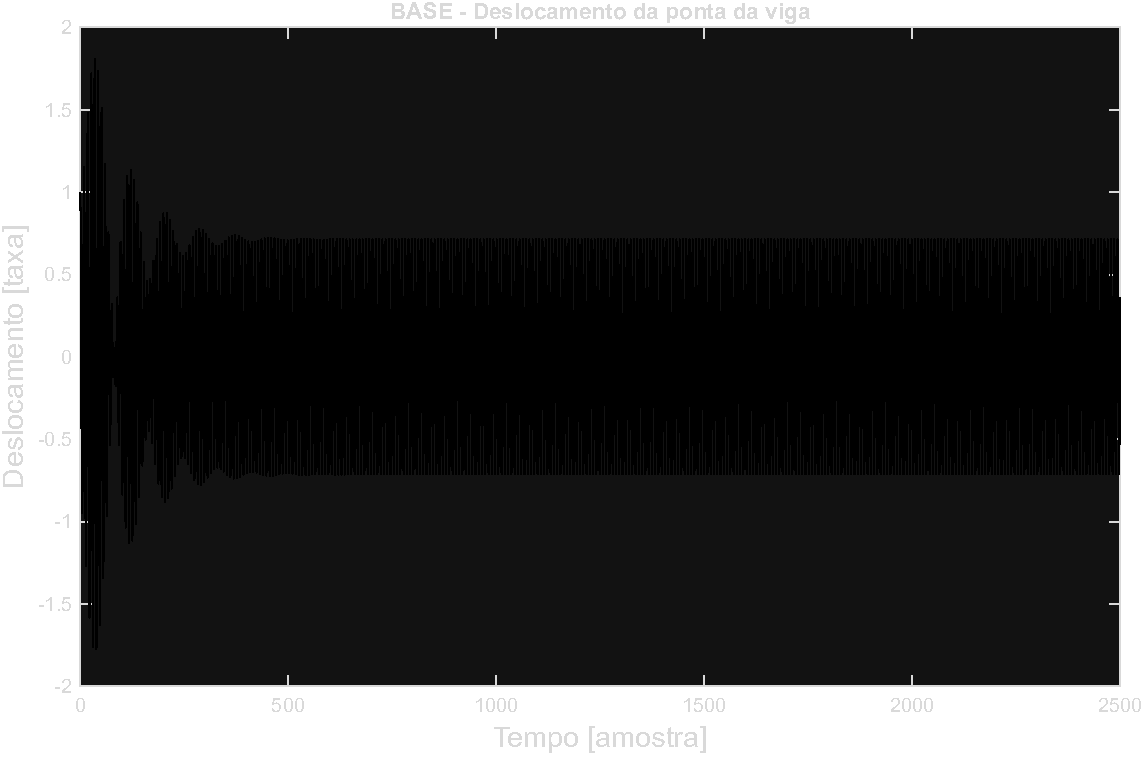
\includepdf[pages=-,pagecommand={},width=\textwidth]{../figuras/aula1_graficos.pdf}

\section{Conclusão}

As três modificações propostas permitiram observar, de forma isolada, o
efeito de três grandezas físicas distintas sobre o mesmo sistema linear
de captação de energia: o amortecimento mecânico ($\zeta$), a frequência
de excitação ($\Omega$) e a amplitude da excitação ($f$). O amortecimento
reduz a potência captada, enquanto a operação próxima à ressonância e o
aumento da amplitude de excitação a elevam substancialmente. Em nenhum
dos casos o sistema deixou de ser estável, reforçando que, para o modelo
linear, o comportamento caótico não está presente, ele surgirá apenas
ao se introduzir não linearidades no sistema.

\end{document}
